% !TeX program = lualatex
% !TeX spellcheck = en_GB
\documentclass[a4paper,10pt]{article}

\usepackage{array}
\usepackage[%
    style=authoryear,
    isbn=false,
    url=false,
    backend=bibtex,
]{biblatex}
\usepackage{enumitem}
\usepackage{etoolbox}
\usepackage{float}
\usepackage{fontawesome5}
\usepackage{fontspec}
\usepackage[margin=1in]{geometry}
\usepackage{graphicx}
\usepackage{lua-ul} % underline for lualatex
%\usepackage{soul} % for underlines, doesn't work with superscript
\usepackage{tabularray}
\UseTblrLibrary{booktabs}
\usepackage{textcomp}
\usepackage{titlesec}
\usepackage{xcolor}
\usepackage{xparse}
\usepackage{hyperref}


% Settings
\hypersetup{%
    colorlinks,
    urlcolor=magenta5,
}
\titleformat{\section} % command
    [display] % shape
    {\Large\sectionfont\color{sectioncolor}} % format
    {} % label
    {0em} % sep
    {} % before-code
    [\vspace{-0.8em}\rule{\textwidth}{1pt}] % after-code
\titlespacing*{\section}{0em}{-1.5em}{0em}
\setlist[itemize]{
    % vertical spacing
    topsep=0em,
    itemsep=0em,
    % horizontal spacing
    %labelindent=0em,
    leftmargin=1em,
    labelsep=3pt,
}
\setmainfont{IBMPlexSans}[%
	Extension=.otf,
	UprightFont=*-Regular,
	BoldFont=*-SemiBold,
	ItalicFont=*-TextItalic,
]
\setmonofont{RobotoMono}[%
	Scale=MatchLowercase,
]
\newfontfamily{\Roboto}{Roboto}
%\newfontfamily{\ClearSans}{Clear Sans}
\def\sectionfont{\Roboto}
\def\projectfont{}
\def\infofont{\sectionfont}
\definecolor{projectcolor}{HTML}{7E1717}
\definecolor{sectioncolor}{HTML}{E55807}
\definecolor{infocolor}{HTML}{7E1717}
\SetTblrStyle{foot}{font=\footnotesize\vspace{-0.5em}}



% openfoam related
\newcommand{\of}{\href{https://openfoam.org/}{\texttt{OpenFOAM}}}
\newcommand{\rcf}{\texttt{rhoCentralFoam}}
\newcommand{\rcfrk}{\texttt{rhoCentralFoamRK3}}
\newcommand{\apupfrk}{\texttt{ausmPlusUpFoamRK3}}
\newcommand{\apup}{AUSM\textsuperscript{+}-up}
% other softwares
\newcommand{\feap}{\href{https://www.cs.cornell.edu/~bindel//blurbs/feap.html}{\texttt{FEAP}}}
% other commands
\newcommand{\duration}[1]{\hfill \textcolor{gray}{\small \faCalendar[Regular]{} #1}}
\NewDocumentCommand{\education}{%
	m % degree
	m % institute
	m % timeline/duration
	o % additional info (thesis title, CPI etc.)
}{%
	{\bfseries#1} | #2\duration{#3}
	\IfNoValueF{#4}{\\#4}
}
\NewDocumentCommand{\HangingList}{% a hanging list created using tblr environment
	m % colspec
	O{} % additional options to tblr,
	m % tblr content
}{%
	\begin{tblr}{%
		colspec=#1,
		rowsep=0.5pt,
		colsep=2pt,
		rows={m},
		row{odd}={black!3},
		#2,
	}
		#3
	\end{tblr}
}
\ExplSyntaxOn
\NewDocumentCommand{\highlight}{%
    O{1} % highlighting level
    m % the word to highlight
}{%
    \int_case:nnF{#1}{%
        {1}{\textbf{#2}} % highlight level 1
        %{2}{\emph{#2}} % level 2
        %{3}{\underline{#2}}
    }
    {#2} % default
}
\ExplSyntaxOff
\NewDocumentCommand{\project}{% prints out project details
    m % project name/title
    m % project supervisor
    m % venue
    m % duration
}{%
    {%
    	\projectfont
        {\textcolor{projectcolor}{#1}}\duration{#4}\\%
        {#2 $\vert$ #3}
    }
}
\renewcommand{\labelitemi}{\textcolor{gray}{\small\faJira}}
\renewcommand{\labelitemii}{\textcolor{gray}{\faGenderless}}



\addbibresource{../publications/publications.bib}



\begin{document}
\setlength{\intextsep}{0.1em}
\setlength{\textfloatsep}{0.1em}
\pagenumbering{gobble}
{
    \noindent\color{infocolor}\infofont
%    \begin{minipage}{0.07\textwidth}
%        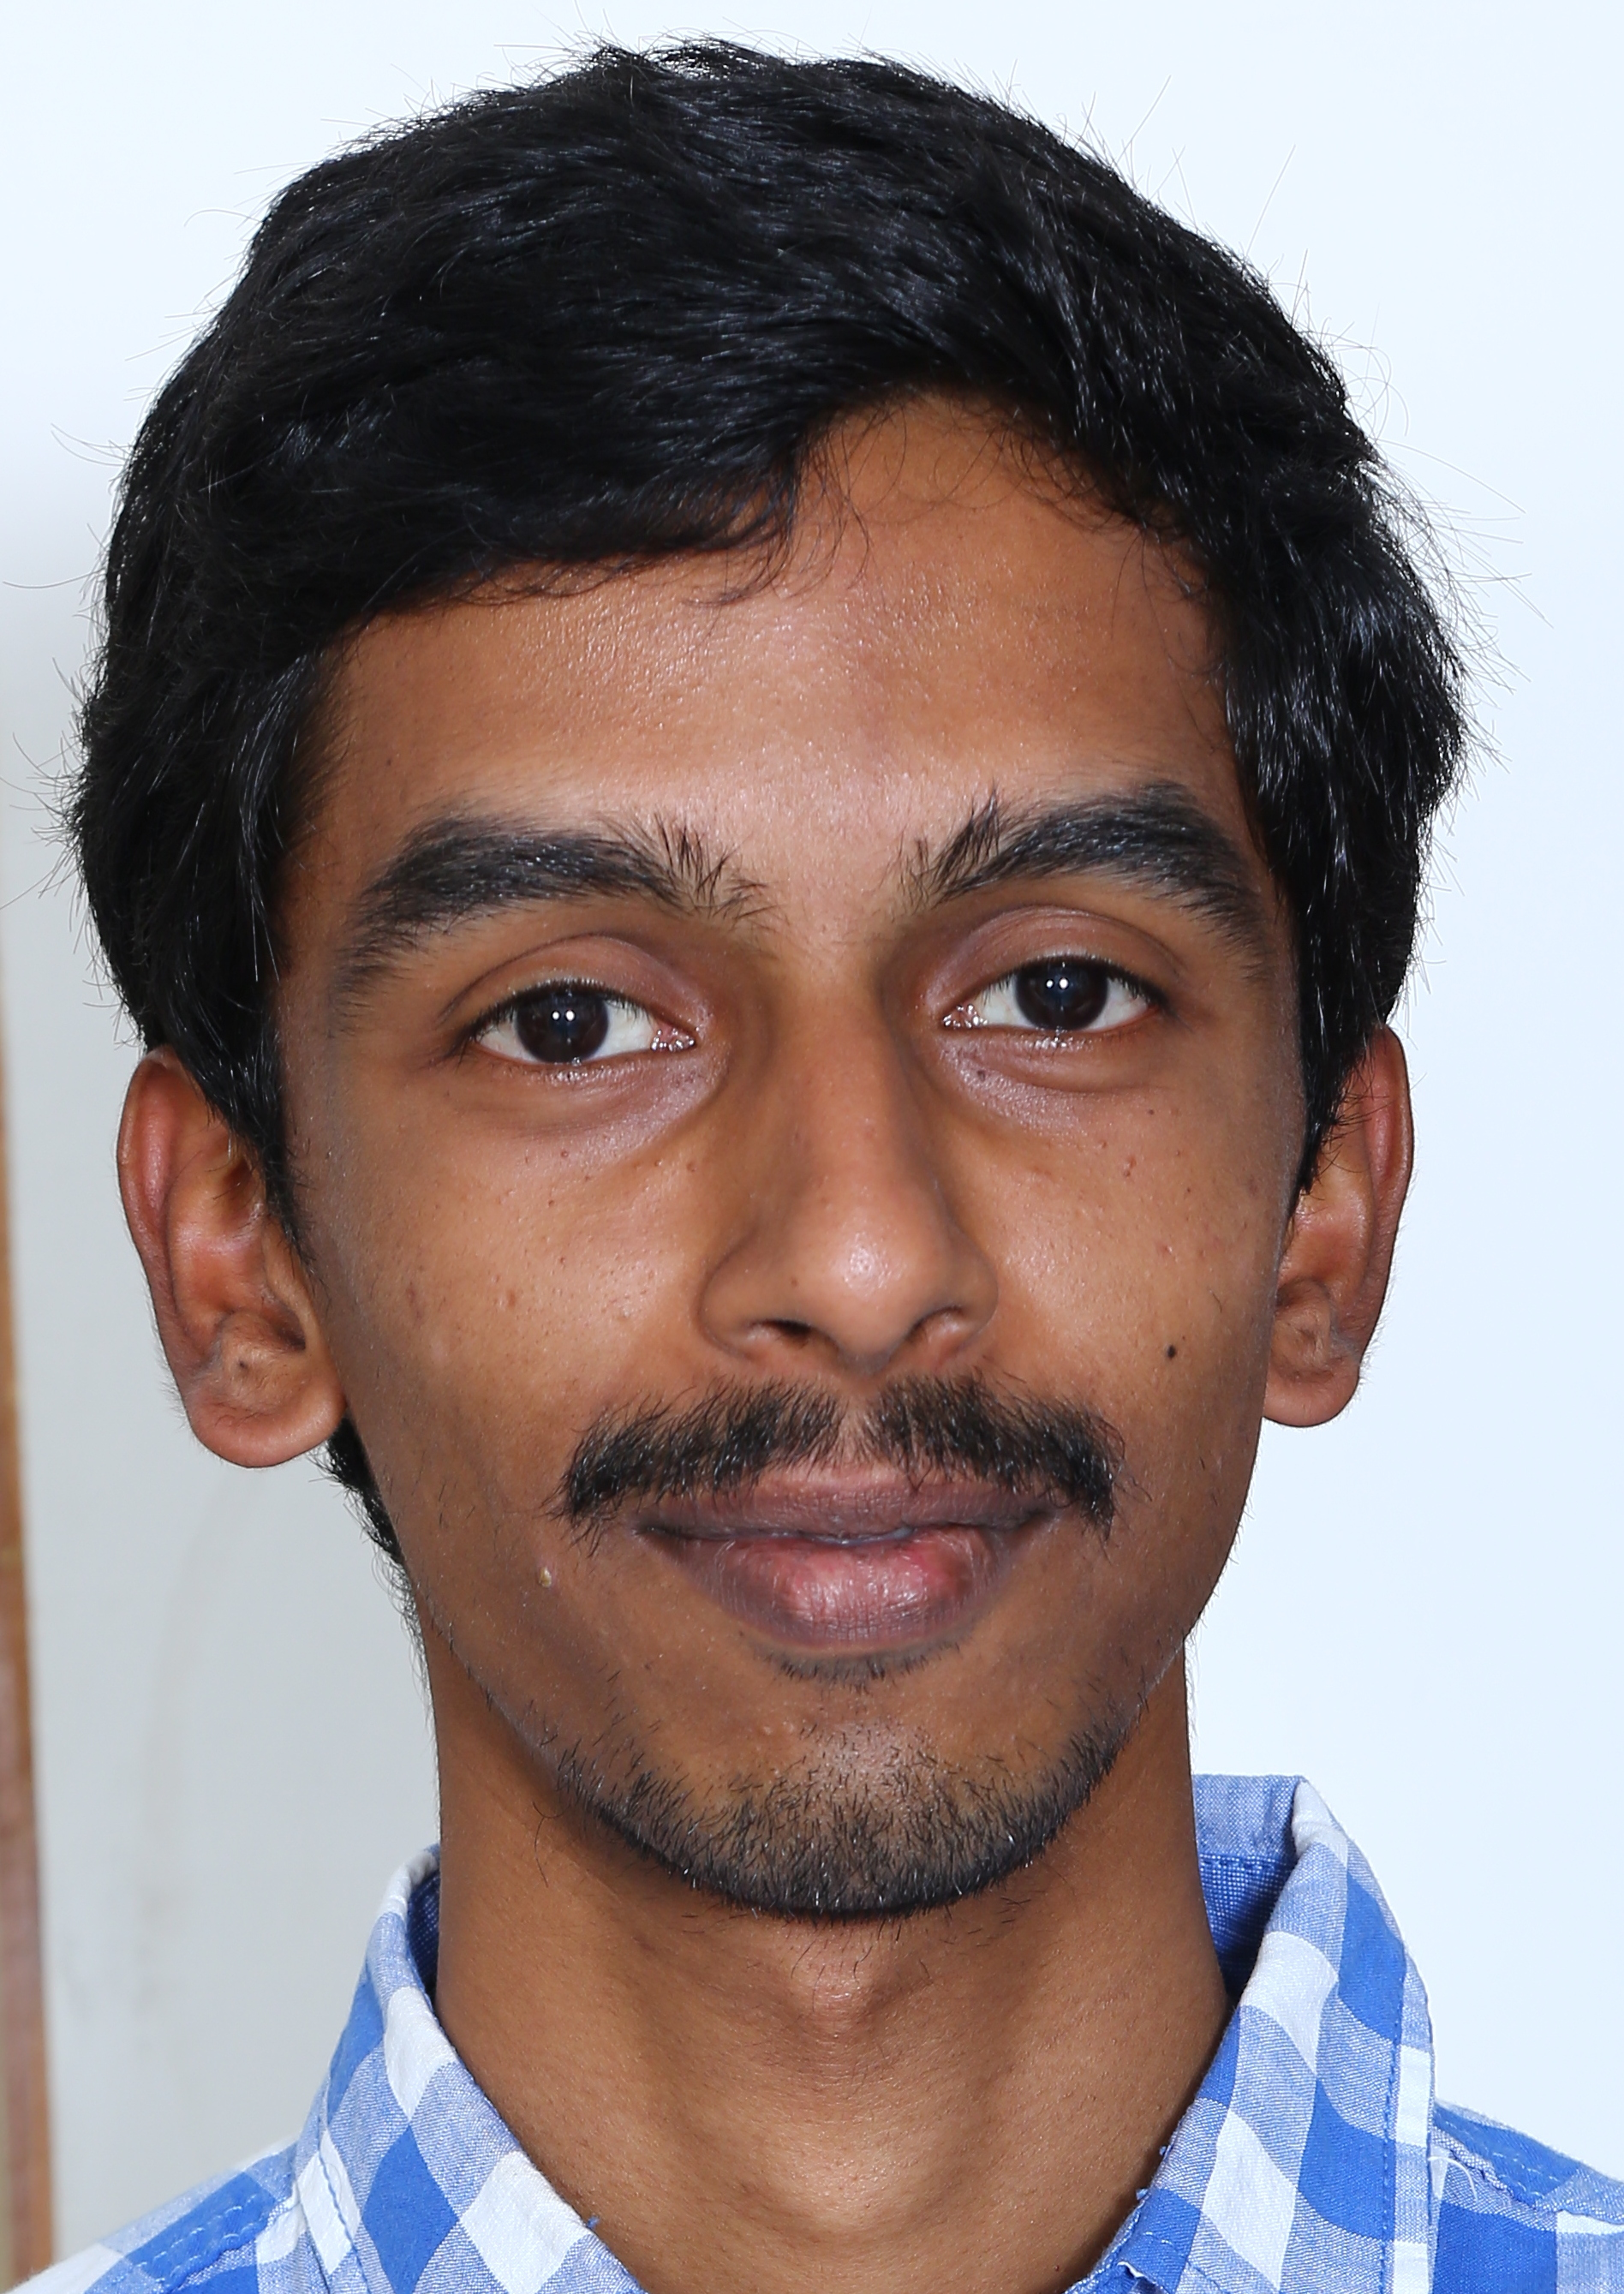
\includegraphics[width=\linewidth]{photo}
%    \end{minipage}%
%    \hspace{1em}
    \begin{minipage}{0.8\textwidth}
    	{\Large\bfseries Potluri Vachan Deep}\\[0.5em]
    	{\large Ph.D. research scholar, IIT Bombay}\\[0.55em]
    	{
   			\faEnvelope[regular]{} \texttt{vachanpotluri1997@gmail.com} \quad
   			\faPhone{} +91-773-869-5898 \quad
   			\faLinkedin{} \href{https://www.linkedin.com/in/vachan-potluri-a202a4237/}{Vachan Potluri}
   		}\\
        {\faGlobe{} \url{https://vachan-potluri.github.io/}}
    \end{minipage}%
}
\vspace{0.5em}
%%%%
\section{Education}
\education{Ph.D. Mechanical Engineering}{IIT Bombay}{Jul `18 -- Dec `23*}[%
	\HangingList{XX[5]}{%
		Thesis title & Development and analysis of discontinuous Galerkin computational framework for high order simulation of hypersonic shock-boundary layer interaction\\
		CPI & 9.86\\
		Key electives & Galerkin Methods for Fluid Dynamics, High Performance Scientific Computing, Magnetohydrodynamics and its engineering applications
	}
]\\[0.5em]
\education{B.Tech. Mechanical Engineering}{IIT Bombay}{Jul `14 -- Jul `18}[%
	\HangingList{XX[5]}{%
		CPI & 9.72\\
		Key electives & Computational Fluid Dynamics and Heat Transfer, Essentials of Turbulence, Finite Element and Boundary Element Methods, Fuels and Combustion, Numerical Methods for Conservation Laws\\
	}
]
%%%%
\section{Related experience}
\begin{itemize}
	\item \project{Development of high resolution schemes for compressible flows in \of}%
		{Prof. Bhalchandra Puranik}%
		{IIT Bombay}%
		{Dec `16 -- Apr `18}
	\begin{itemize}
		\item \highlight{Modified an existing solver} \rcf{} to use \highlight[2]{TVD-RK3 time integration} scheme
		\item \highlight{Developed a new solver} \apupfrk{} that uses \highlight[2]{\apup{} flux scheme} along with RK3 time integration scheme
		\item \highlight{Performed a comparative study} using these two solvers by conducting simulations of several 1D and 2D test cases to draw useful conclusions
	\end{itemize}
\end{itemize}
%%%%
\section{Other experience}
\begin{itemize}
	\item \project{Unified 2D Finite Element}
	{Prof. Parag Tandiya}
	{IIT Bombay}
	{Mar `18 -- Apr `18}
	\begin{itemize}
		\item \highlight{Implemented a subroutine} in FORTRAN77 library \feap{} for a \highlight[3]{new combined Plane Stress, Plain Strain and Axi--symmetric linear elasto--static element}, and validated the subroutine using several simple test cases
	\end{itemize}
	\item \project{Stair climbing wheel chair}
	{Prof. Shantanu Tripathi}
	{IIT Bombay}
	{Jul `17 -- Dec `17}
	\begin{itemize}
		\item \highlight{Proposed a mechanism} for a \highlight[2]{passive wheel chair} capable of \highlight[2]{climbing stairs} using the \highlight[3]{force provided by a companion}
		\item \highlight{Built} a \highlight[2]{full scale basic functioning prototype} \highlight[3]{within 2 months} constraining to the alloted budget and resources
		\item \highlight{Tested the prototype} on 2 different stair geometries and demonstrated it's effectiveness to Mechanical Engineering Department faculty, staff, and other students
	\end{itemize}
	\item \project{GE90 HPC airfoil durability analysis}
	{Mr. Nageswara Ganji, Mr. Devesh Ojha}
	{John F. Welch Technology Center, General Electric}
	{May `17 -- Jul `17}
	\begin{itemize}
		\item \highlight{Modified} the \highlight[2]{mesh} of existing GE90-115B high pressure compressor stage-9 rotor blade, to model
		\begin{enumerate}
			\item Three types of \highlight[2]{damaged blades} by \highlight[3]{making notches} at different locations on the leading edge
			\item A \highlight[2]{defectively manufactured blade} by \highlight[3]{changing thickness of leading edge} according to manufacturing tolerance
		\end{enumerate}
		\item \highlight{Generated Campbell Diagrams} by \highlight[2]{simulating the vibration response} and \highlight{recalculated fatigue factor of safety}\ at critical locations of undamaged, damaged and defected blades for \highlight[2]{3 different materials}
	\end{itemize}
\end{itemize}
%%%%
\section{Publications}
\nocite{potluriPuranikBodi2022,potluriPuranikBodi2023}
\printbibliography[%
heading=none,
]
%%%%
\section{Scholastic Achievements}
\begin{itemize}
	\item \highlight{Stood 2nd in Department} out of more than \highlight[2]{150 students} in B.Tech. \duration{May `18}
	\item \highlight{Scored 829} in \highlight[2]{Graduate Aptitude Test in Engineering (GATE) 2018} \duration{Mar `18}
	\item \highlight{Secured All India Rank 129} in \highlight[2]{JEE Advanced 2014} in general category \duration{May `14}
	\item Awarded \highlight{Kishore Vigyanik Protshahan Yogana} (KVPY) fellowship by Indian Institute of Science (IISc), Bangalore \duration{Dec `13}
	\item \highlight{Secured position among top 1\%\ students} of former Andhra Pradesh who participated in \highlight[2]{National Standard Examination in Physics (NSEP)} \duration{Dec `13}
\end{itemize}
\end{document}